\chapter[Zmogljivst Beowulf gruče Raspberry Pi računalnikov (G. Vitek,  Ž. Palčič, M. Smerkol)]{Zmogljivst Beowulf gruče Raspberry Pi računalnikov}
\huge Gregor Vitek, Žan Palčič, Maj Smerkol\\
\normalsize
\bigskip

%%%%%%%%%%%%%%%%%%%%%%%%%%%%%%% fukni ven po potrebi
\section{Slike}
Slike pripravite v EPS formatu. Na sliki  \ref{fig:poglavje2_ac} je za zgled navedena ena slika Petrijevih mrež.

\begin{figure}[htbf]
\begin{center}
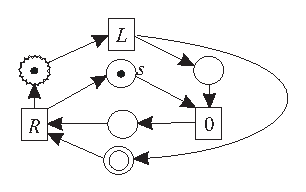
\includegraphics{poglavje2_ac}
\end{center}
\caption{Model popravljive entitete, ki za servisiranje zahteva prisotnost resursa $s$.}
\label{fig:poglavje2_ac}
\end{figure} 
%%%%%%%%%%%%%%%%%%%%%%%%%%%%%%%%%%

%%%%%%%%%%%%%%%%%%%%%%%%%%%%%%%%%%%%%%%%%%%%% naš tekst

\section{Uvod}

Na spletu lahko najdemo že opravljene znane benchmarke\cite{Benchmarks}, ki ocenjujejo določene lastnosti oblačnih sistemov (S2). Tu lahko najdemo podatke o procesni moči sistema, ki ga dobimo v uporabo, količini pomnilnika na takšnem sistemu in zmogljivosti opravljanja nekaterih znanih testov, kot so naprimer urejanje velike količine podatkov. Te meritve, ki jih lahko preberemo med že opravljenimi testi, pa ne kažejo na zmogljivost neke določene storitve, kot jo doživlja uporabnik, ampak samo povejo, kako zmogljiva je strojna oprema, ki jo dobimo na voljo. Končnega uporabnika storive pa ponavadi zanima predvsem hitrost odzivanja, ki je odvisna od več parametrov.
Med slednje spadajo hitrost in latenca povezave od naprave uporabanika (end point) do fizične lokacije oblačne storitve ali strežnika, velikost poslanega zahtevka, hitrost odbelave zahtevka, hitrost in latenca poslanega odgovora iz oblaka ali strežnika proti uporabniku in drugo. Pri tem lahko lahko nekatere storitve implementiramo na tak način, da uporabnik verjame, da je odzivni čas veliko manjši, kot dejansko je (naprimer shranjevanje datotek na disk v oblaku). Na končno uporabnikovo izkušnjo hitrosti pa vpliva tudi zmogljivost naprave, ki predstavlja njegovo dostopno točko. 

Kot omenjeno zgoraj se na spletu najdejo seznami spletnih sistemov, ki jih lahko uporabniki med seboj primerjajo. Primerjajo lahko rezultate za različne parametre kot so hitrost procesorja pri računanju s plavajočo vejico ali celimi števili, hitrost prenosa pri branju podatkov oz. pisanju na pomnilnih enotah, hitrost prenosa podatkov lokalno znotraj oblačne storitve in drugo. Pri testiranju teh parametrov se lahko uporabi različna orodja kot so SPEC CPU 2006, Test Harness, TeraSort, Geekbench in še mnogo drugih. Pri sami izbiri programov se moramo osredotočiti tudi na bremena, ki jih lahko s posameznim programom definiramo in tako testiramo željene parametre. Ključen kriterij poleg kakovosti storitev in definiranje bremen je tudi cena. Zaželjeni so prosto dostopni oz. zastonjski progami. 

Pri testiranju spletnih strežnikov (S1) uporabnika navadno  zanima število zahtev, ki jih strežnik obdela, latenca oz. čas odziva strežnika za novo povezavo ali zahtevek, in količina prenesenih podatkov v sekundi, glede na različne parametre (velikost, shranjevanje v predpomnilnik, različna pasovna širina). Za izvajanje stresnih testov se na spletu nahaja veliko orodij, ki lahko pridejo v pomoč (Apachech, Apache JMeter, Curl-loader, OpenSTA …). 

\subsection{Znanje}

Sistem, ki ga bomo testirali, smo izbrali na podlagi svojega znanja in zanimanja. 
Člani te skupine imamo predznanje iz arhitekture in organizacije računalniških sistemov, kot so procesne enote, pomnilniška hierarhija in vhodno/izhodne naprave. Poznamo tudi paralelno programiranje na različnih platformah v jeziku C, kar bi nam lahko pomagalo pri optimizaciji določenih storitev. Imamo predznanje iz strežniških arhitektur in osnov spletne komunikacije. Imamo tudi omejene izkušnje uporabe PaaS (platform as a service) za postavitev spletnih strani in postavitve podakovnih baz na teh strežnikih. Nimamo pa izkušenj s testiranjem in merjenjem zmogljivosti katerega koli on naštetih modelov.

\begin{figure}[htbf]
\centerline{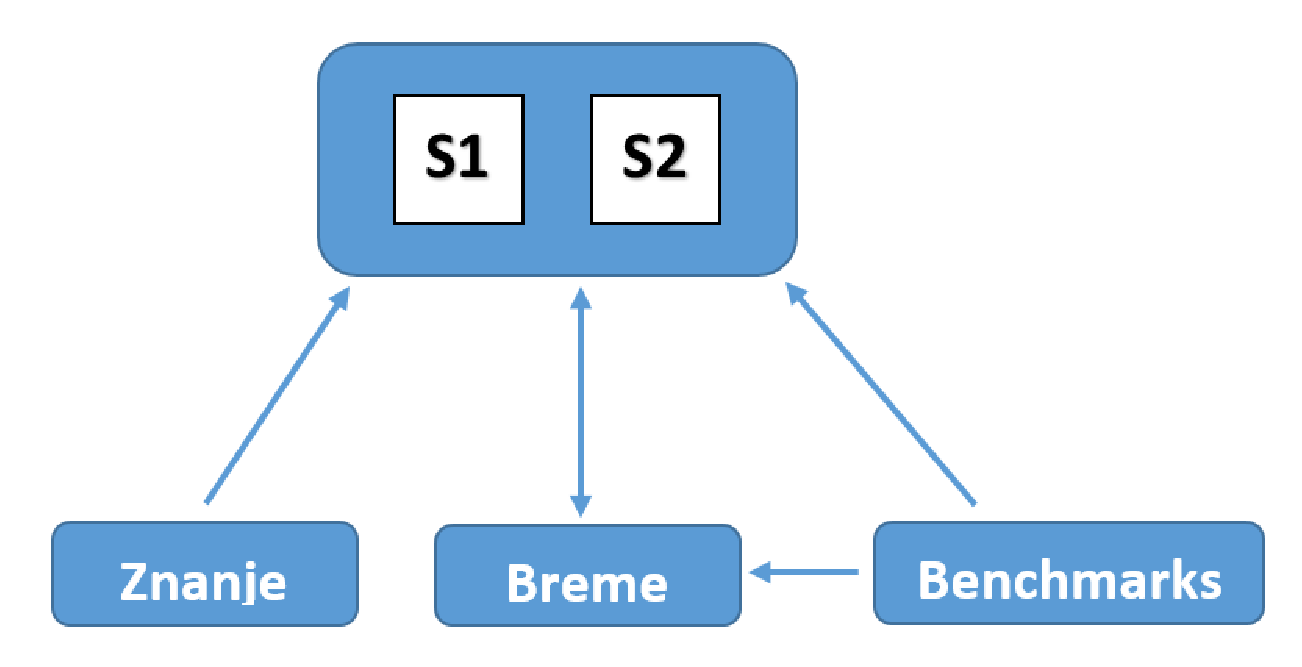
\includegraphics[scale=0.5]
{vzorec.eps}}
\caption{Odvisnost izbire S1 in S2 glede na podane atribute.}
\label{fig:miselni}
\end{figure}
\subsection{Benchmarks}

\subsection{Izbira ciljnih sistemov}

Za ciljni sistem bi lahko izbrali kakšnega od večjih ponudnikov oblačnih storitev kot so Google Cloud, Amazon web service, Microsoft Azure, lahko tudi kakšne manjše kot so Rackspace. Večina teh ponudnikov ima omejene zastonjska testna obdobja, med katerimi bi lahko izvedli meritve.
Ker imamo dostop do računalnika Raspberry Pi \footnote{http://www.raspberrypi.org/} in predvsem zastonjskih verzij oblačnih storitev, nas zanima primerjava med temi platformami. Raspberry Pi je računalnik, ki stane okrog 30 evrov in ne porabi praktično nič elektrike, v zameno pa ponuja primerno majhno zmogljivost. Ne plačljive oblačne storitve pa so močno časovno omejene ali pa ponujajo prav tako zelo majhne zmogljivosti.
Zaradi naših predznanj lahko storitev za strežnik, katerega ustroj in delovanje poznamo, bolje optimiziramo, kot oblačno storitev, kar je prav tako vredno preveriti.

Ker pa je iplementacija optimizirane storitve in postavtev lastne gruče relativno zahtevno opravilo, mi pa imamo na voljo omejen čas, smo se odločili za testiranje zmogljivosti gruče računalnikov Raspberry Pi. Le ti so se v zadnjem času zaradi nizke cene na mnogih področjih računalništva začeli uporabljati. Nas zanima, ali so računalniki takšnega tipa primerni tudi za uporabo na področjih, ki zahtevajo računsko moč. Na podlagi izmerjenih rezultatov lahko primerjamo zmogljivost z drugačnimi sistemi, na katerih so meritve že opravljene. Prav tako lahko nadaljujemo raziskovanje na tem podrpčju z poskusom optimizacije enake storitve na drugačnem sistemu opravimo v prihodnosti.

\subsection{Breme in cilj primerjave}

Za storitev, ki jo bo naša gruča ponujala, smo izbrali manipulacijo nad frekvenčnim spektrom avdio datotek. To pomeni, da smo implementirali porazdeljen algoritem FFT, ki pretvori datoteko iz vzorčnega prostora v frekvečni spekter, nato nad temopravimo preprosto operacijo naprimer zamik v višje frekvence, nato pa z inverznim FFT naredimo spet datoteko v vzorčnem prostoru.

Bremena so tako različno velike zvočne datoteke. Ker naš spletni strežnik, ki to storitev ponuja, sprejme eno ali več datotek, testiramo tudi izvajanje večih instanc algoritma hkrati.

Cilj primerjave je ugotoviti, ali je računalnik Raspberry Pi primeren za postavitev gruče, ki bo izvajala računsko zahtevne storitve. Da bi to ugotovili, moramo primerjati čas izvajanja na procesorju, čas latence oddaljenega sistema prek medmrežja in čas pošiljanja podatkov po gruči.

\section{Sistem}

Naš sistem je gruča računalnikov, narejena po vzoru Beowulf gruč. Namenjena je zaganjanju porazdeljenih programov. Trenutno sta v mrežo povezana dva računalnika Raspberry Pi, model 1B in model 1B+. Povezani so v gručo s pomočjo knjižnjice MPI. Do njega imamo SSH dostop tudi z zunanjega omrežja. Storitev je dostopna prek strežnika, ki smo ga implementirali sami.

\begin{figure}[H]
\centerline{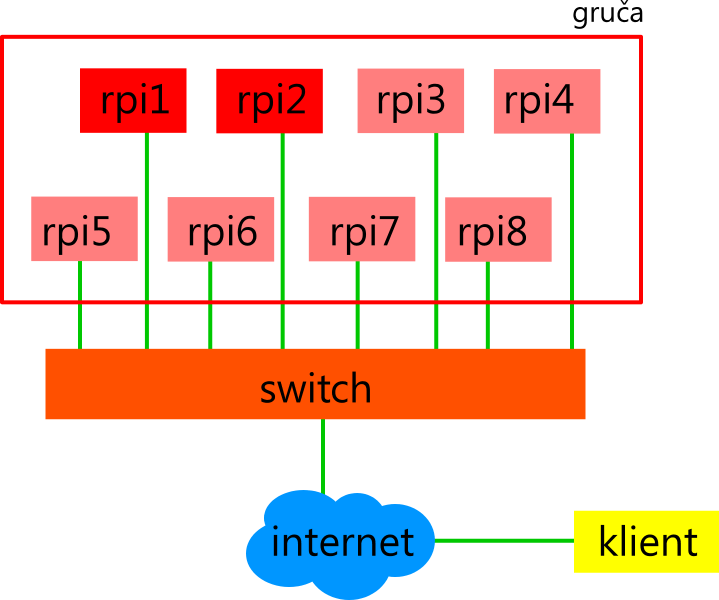
\includegraphics[scale=1.5]
{shemaSistema.png}}
\caption{Shema sistema. Rdeči kvadrati so računalniki Raspberry Pi, bledo rdeči še niso dodani.}
\label{fig:gruca}
\end{figure}

Do tega sistema dostopamo s klienti, ki so izven lokalnega omrežja. Gručo uporabljamo kot računski strežnik, ki po zahtevi klienta izvaja porazdeljeno hitro Fourierjevo transformacijo. Klient prek omrežja pošlje podatke v obliki glasbene datoteke, gruča pa podatke sprejme (to stori strežnik, ki teče na master računalniku gruče) in izvajanje algoritma porazdelil prek vseh računalnikov v gruči, vključno s sabo.

V začetku smo testirali dostop do gruče od zunaj in delovanje sistema MPI na računalniku rpi1. To smo storili tako, da smo na njem poganjali z MPI implementiran algoritem porazdeljeni Quicksort (porazdeljeno hitro urejanje\footnote{http://en.wikipedia.org/wiki/Quicksort\#Parallelization}).

Pri povezovanju Raspberry Pi-jev v gručo smo uporabili Message Passing Interface(MPI), ki je standard za izmenjevanje sporočil med računalniki oz. procesih v več-računalniških sistemih, gručah in delovnih postajah. Omogoča komunikacijo točka-točka, skupinske komunikacije, spremljanje delovanja in tudi spreminjanje topologije za posamezen program. MPI je standard, ki omogoča velik nabor funkcij, vendar za uporabo standarda ni potrebno poznati vseh. Pri sami komunikaciji računalniki med seboj uporabljajo implementacijo MPICH2 \cite{Mpich},
ki je zelo razširjena programska knjižnica poleg tega pa je enostavna za vzpostavitev in uporabo. Na vsakem računalniku je implementacija 
MPICH2 in datoteka (machinefile)\cite{Gruca} v kateri so zapisani IP naslovi sodelojočih(sosednjih) lokalnih računalnikov, na katere se delo porazdeli.

Implementirali smo porazdeljeni algoritem FFT, ki se izvaja na gruči. 

\subsection{Implementacija storitve}

V gručo smo dodali več računalnikov, da je prava gruča, ne le en računalnik, na katerem teče MPI. Raspberry Pi smo pripravili na delovanje v gruči tako, da smo klonirali sliko datotečnega sistema. Potrebni so bili popravki v konfiguraciji omrežja in sprememba hostname-a vsakega računalnika, po tem gruča deluje brez težav.

Implementirali smo storitev, ki zvočno datoteko pretvori v binarno s pomočjo knjižnjice \texttt{libsndfile}\cite{Audio}. Testiranje smo izvedli z zvočno datoteko, veliko približno 8 miljonov vzorcev (okrog 3 minute zvoka). Program na enem jedru teče zelo počasi. Ni se izpolnil strah, da bi algoritem tekel prehitro, da bi se izplačalo ga poganjati na gruči. Imeli smo nekaj težav s kodiranjem datoteke nazaj v zvočno datoteko.

Pretvorbo izvjamo z rekurzivnim algoritmom FFT. Implementacija je zaradi uporabe razreda ValArray iz knjižnjice STL počasna, če je prevanjanje izvedeno z Microsoft Visual Studio prevajalnikom. Program, ki se izvaja na gruči, na kateri teče Linux (distribucija Arch Linux), je preveden s prevajalnikov gcc, ki se v tem primeru obnaša veliko bolje - koda se izvaja hitreje.

\vspace{10pt}

Implementirali smo strežnik, ki sprejema zahtevke z eno ali več datotekami in nato odgovori. Implementirali smo tudi klienta, ki pošilja zahtevek z eno ali več datotekami in sprejme odgovor strežnika.

Program, ki izvaja manipulacije frekvenčnega spektra, upošteva lastnosti hitre Fourierjeve transformacije in pravilno obdeluje zvok. Zavržemo del frekvenčnega spektra, ki je zrcalna slika relevantnega dela. Transformacije, ki jih izvajamo na preostanku so zato bolj smiselne in se obnašajo kot pričakovano.

\vspace{10pt}

% povezovanje v enoten sistem

\section{Meritve}

Naš problem predstavlja veliko računsko breme gruči ampak relativno majhno breme za prenos podatkov prek omrežja. Na enem vozlišču traja obdelovanje 5 sekund zvoka okrog 40 sekund. Algoritem je hitrostnega razreda $O(n log n)$.

Zaradi tipa problema in bremena nas zanimajo časi računanja (procesiranja na gruči, wall-clock time, v odvisnosti od števila uporabljenih vozlišč in velikosti bremena), prenosa podatkov na in iz gruče (latenca omrežja - čas prenosa je najbrž zanemarljiv, saj so datoteke velike med 1MB in 10MB), latence prenosa podatkov med vozlišči v gruči (da vidimo, ali je paralelizacija na gruči primerna ali bi bilo bolje uporabljati paralelizacijo na več jedrih ali podobni arhitekturi) in največje število datotek, ki jih lahko obdeluje hkrati, preden se gruča ali deli nje sesujejo.

Izmerjeni časi: 
\begin{itemize}
\item Procesiranje, 1 vozlišče, n = 5s: približno 40 sekund
\item Procesiranje, 2 vozlišči, n = 5s: približno 20 sekund
\item Procesiranje, 3 vozlišča, n = 5s: približno 19 sekund
\end{itemize}

Razlika med 2 in 3 vozlišči je premajhna, da bi lahko sklepali na pohitritev. Zaradi tipa algoritma (FFT se rekurzivno deli vedno na dva dela, zato deluje dobro le, če uporabljamo $2^n$ paralelnih niti.

Ker za dovolj velik $n$ velja $nlog(n) > nlog(n/m)*m$, je hitrost reševanja problem večja, če rešujemo več manjših problem, kot enega velikega. To je razlog, da ne porazdeljujemo po gruči po drevesu razcepa podatkov, ki ga izvaja FFT, ampak razdelimo vse podatke na $m$ delov in nato odbelujemo vsakega posebej, pri čemer je $m$ število računalnikov v gruči. To je slaba rešitev za zelo velik $m$ ali zelo majhne zahtevke, saj bi se lahko poznala izguba kvalitete zvoka, ki jo to prinese. Razlika se na normalnih zahtevkih in našem $m$ sicer ne pozna. Takšen pristop se uporablja tudi v praksi, predvsem kadar se izvaja transformacije v realnem času (sproti).

\section{Načrt za naprej}

Še vedno nismo opravili vseh meritev, ki jih nameravamo. V tem tednu bomo izvajali eksperimente z različno velikimi bremeni in v različnih okoliščinah. Za rezultat meritev bomo upoštevali najmanjšo, največjo in povprečno meritev.


%%%%%%%%%%%%%%%%%%%%%%%%%%%%%%%%%%%%%%%%%%%%%%%%%%%

\section{Citiranje}
V priloženi datoteki mro.bib imate vzorce, kako kakšne reference (vire) zabeležiti v taisto datoteko. V viru \cite{sch1} najdemo kar nekaj zanimivosti o Petrijevih mrežah.

